\documentclass[a4paper]{article}
\usepackage{cmap}
\usepackage{url}
\usepackage[utf8]{inputenc}
\usepackage[russian]{babel}
\usepackage{graphicx}
\graphicspath{{img/}}
\frenchspacing
\begin{document}
\author{В.\,В.~Бочаров\\\small Mathlingvo\\\small\tt bocharov@opencorpora.org\and С.\,В.~Бичинева\\\small СПбГУ\\\small\tt\ bichineva@opencorpora.org\and Д.\,В.~Грановский\\\small Mathlingvo\\\small\tt grand@opencorpora.org\and Н.\,А.~Остапук\\\small СПбГУ\\\small\tt\ nataxan90@gmail.com\and М.\,Е.~Степанова\\\small СПбГУ\\\small\tt\ mariarusia@gmail.com}
\title{Инструменты контроля качества данных в проекте Открытый корпус}
\date{}
\maketitle
\begin{abstract}
Открытый корпус (OpenCorpora)~--- проект по созданию размеченного корпуса текстов на русском языке, доступного для исследователей в полном объеме и редактируемого пользователями. В статье рассматриваются инструменты, предназначенные для обеспечения качества морфологической разметки.
\end{abstract}
\section{Введение}
В настоящее время проблема отсутствия корпусов текстов на русском языке, в том числе размеченных, казалось бы, не стоит. Более того, некоторые корпусы доступны в Интернете (см. обзор в~\cite{reznikova05}), что, на наш взгляд, существенно повышает их ценность для лингвистического сообщества. Насколько можно судить, под доступностью в Интернете обычно понимается наличие некоторого интерфейса, посредством которого пользователь может производить поиск в корпусе по разным параметрам. Безусловно, это открывает большие возможности для разнообразных теоретических исследований в области языка, для которых требуется анализ контекстов употребления слов, их частотности и~т.\,д. Однако, для использования корпуса в качестве ресурса для обучения или тестирования прикладных разработок~--- например, морфологических парсеров или систем снятия неоднозначности~--- этого недостаточно, поскольку в таких случаях требуется доступ непосредственно к размеченным текстам, а не к результатам поиска по ним. Получить такую разметку из существующих корпусов в принципе возможно, однако это связано со значительными трудностями~--- как технического, так и административного или лицензионного характера.

Такое положение вещей послужило мотивацией для начала проекта <<Открытый корпус>> (OpenCorpora). В его рамках предполагается создание размеченного (в ближайшем будущем морфологически, впоследствии также синтаксически и семантически) корпуса русскоязычных текстов, содержимое которого доступно всем желающим под свободной лицензией, а разметка осуществляется сообществом пользователей. Эта модель работы уже зарекомендовала себя во многих проектах, самый известный из которых, вероятно, Википедия~\cite{ruwiki}. Использование этой модели для получения лингвистических данных обсуждается в нескольких работах (например, в~\cite{munro10} и \cite{wang10}), и есть указания на то, что качество разметки сравнимо с результатами, полученными традиционным способом, а в некоторых случаях превосходит их. Целью проекта OpenCorpora является создание качественной разметки, которая могла бы быть использована в дальнейшем при разработке программ для снятия морфологической неоднозначности и иного ПО.

В корпус будут включены тексты, находящиеся в общественном достоянии, и полученные из источников, разрешающих копирование и распространение, т.\,е. использующих лицензию, совместимую с CC-BY-SA. Например, проекты Wikimedia: Википедия и Викиновости~\cite{ruwikinews} и интернет-издание <<Частный Корреспондент>> (www.chaskor.ru). Многие тексты классической русской литературы на данный момент находятся в общественном достоянии и доступны в Викитеке~\cite{ruwikisource}.

Используя краудсорсинг (англ. \textit{crowdsourcing}, \textit{crowd}~--- <<толпа>> и \textit{sourcing}~--- <<использование ресурсов>>) как основной способ создания материалов, необходимо уделить особое внимание качеству результата, т.~к. квалификацию участников трудно проверить заранее. При этом контроль качества желательно сделать настолько автоматизированным, насколько это возможно. Вовлечение специалистов для проверки разметки является наименее приемлемым средством (ввиду высокой стоимости человеческого труда), хотя и необходимым в ряде случаев. Основными инструментами контроля качества морфологической разметки являются модель сочетаемости грамматических помет и морфологический словарь. Оба инструмента используются для описания допустимых сочетаний грамматических помет. При вводе недопустимого сочетания программное обеспечение сгенерирует ошибку. В проекте OpenCorpora в качестве сообщений об ошибках мы используем предупреждения, которые не блокируют действия пользователя. Цель предупреждений~--- обратить внимание на потенциально ошибочный ввод. Окончательное решение о правильности остаётся за пользователем.

Далее в этой статье будет коротко описан сам проект OpenCorpora, устройство его морфологического словаря и модели сочетаемости грамматических помет.
\section{О проекте OpenCorpora}
OpenCorpora~--- это свободно распространяемый на условиях лицензии CC-BY-SA~\cite{cc-by-sa} корпус текстов на русском языке с лингвистической разметкой и программное обеспечение для ее создания и редактирования.

Под лингвистической разметкой понимаются следующие составляющие:
\begin{itemize}
\item графематика: сегментация цепочки знаков на текстоформы, предложения и абзацы;
\item морфология: указание для текстоформ части речи и грамматических признаков, снятие морфологической неоднозначности;
\item локальный синтаксис:
\begin{itemize}
\item указание границ неоднословных сущностей (аналитических глагольных конструкций, сложных сравнительных и превосходных степеней прилагательных, составных числительных, составных союзов, предлогов и частиц, наречных, предикативных и вводных оборотов, имён людей и объектов, дат) и их грамматических характеристик;
\item объединение текстоформ в синтаксические группы (именные, предложные, глагольные, адъективные группы) и указание отношений зависимости в рамках групп;
\end{itemize}
\item лексическая семантика: указание для текстоформы конкретного значения слова.
\end{itemize}

Деление на абзацы берется из источника и введено в основном для удобства добавления текстов, хотя нельзя исключать, что эта информация будет полезна и для исследователя. Деление абзаца на предложения производится автоматически и проверяется пользователем.

Деление предложения на токены также производится автоматически и потом проверяется вручную. Токеном мы считаем минимальную значимую последовательность символов без пробелов. Все токены делятся на словарные (формы, присутствующие в словаре) и несловарные. К несловарным относятся знаки препинания, Интернет адреса, формулы (химические, математические и прочие) и другие сочетания знаков, которые нет смысла помещать в словарь, например, ввиду их неограниченного количества.

Единицей морфологической разметки является токен. Разметка токена состоит из одной или нескольких (в случае омонимии) интерпретаций. Каждая интерпретация обязательно содержит указание на класс токена (словарный, несловарный). Для словарных токенов интерпретация также включает:
\begin{itemize}
\item идентификатор леммы из словаря;
\item часть речи;
\item набор значений обязательных для данной части речи грамматических категорий (например, число для имен существительных);
\item набор меток, обозначающих особенности конкретного употребления словоформы в тексте (например, <<опечатка>>, <<безличное употребление глагола>>).
\end{itemize}

\begin{figure}[h!]
\center{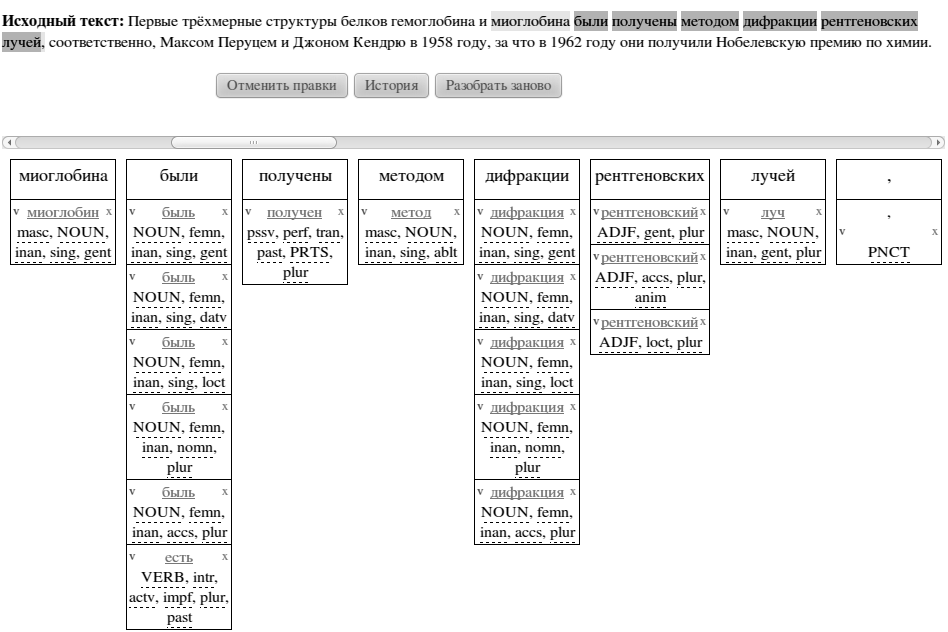
\includegraphics[width=1\linewidth]{2011_Dialog_img1.png}}
\caption{Интерфейс редактора морфологической разметки}
\end{figure}

На рисунке 1 показан фрагмент морфологической разметки предложения в интерфейсе редактора разметки. В верхней части приводится всё предложение целиком. Подсветка в нём указывает на ту часть предложения, разметка которой поместилась в окно по ширине. Сама разметка представлена в виде столбцов, каждый из которых включает все варианты морфологического разбора одной текстоформы. Подчёркнутое слово является гиперссылкой, ведущей в морфологический словарь. Кнопка <<v>> в левой верхней части позволяет отметить вариант как единственный правильный, а все остальные — как неправильные. Кнопка <<x>> отмечает выбранный вариант как неправильный.

Та же информация доступна в формате XML и для текстоформы <<были>> выглядит следующим образом:
\begin{verbatim}
<tfr t="были">
  <v>
    <l id="4342" t="быль">
      <g v="NOUN"/> <g v="femn"/> <g v="inan"/> <g v="sing"/> <g v="gent"/>
    </l>
  </v>
  <v>
    <l id="4342" t="быль">
      <g v="NOUN"/> <g v="femn"/> <g v="inan"/> <g v="sing"/> <g v="datv"/>
    </l>
  </v>
  <v>
    <l id="4342" t="быль">
      <g v="NOUN"/> <g v="femn"/> <g v="inan"/> <g v="sing"/> <g v="loct"/>
    </l>
  </v>
  <v>
    <l id="4342" t="быль">
      <g v="NOUN"/> <g v="femn"/> <g v="inan"/> <g v="nomn"/> <g v="plur"/>
    </l>
  </v>
  <v>
    <l id="4342" t="быль">
      <g v="NOUN"/> <g v="femn"/> <g v="inan"/> <g v="accs"/> <g v="plur"/>
    </l>
  </v>
  <v>
    <l id="52243" t="есть">
      <g v="VERB"/> <g v="intr"/> <g v="actv"/> <g v="impf"/> <g v="plur"/>
      <g v="past"/>
    </l>
  </v>
</tfr>
\end{verbatim}
ПО, разрабатываемое в рамках проекта OpenCorpora, реализует модель веб-приложения, т.~е. запускается на веб-сервере и предоставляет доступ к своим функциям через веб-браузер. Веб-сервер OpenCorpora реализует следующие функции:
\begin{itemize}
\item хранение текстов и разметки с поддержкой истории редактирования;
\item хранение словаря с поддержкой истории редактирования;
\item веб-интерфейс для редактирования словаря и разметки;
\item ПО для контроля качества.
\end{itemize}

На настоящий момент проект находится на стадии разработки ПО для редактирования графематического и морфологического уровня разметки. Текущая версия доступна по адресу \url{http://opencorpora.org}. На момент написания статьи загруженные на сайт данные предназначены для демонстрации функциональности ПО и отладки.
\section{Морфологический словарь}
В проекте OpenCorpora используется морфологический словарь группы АОТ\cite{aot}, адаптированный для задач, связанных с контролем качества разметки. Словарь тесно интегрирован с самим корпусом через числовые идентификаторы лемм, которые являются одним из компонентов морфологической интерпретации текстоформ в разметке. Интеграция морфологической разметки текста со словарём позволяет решить следующие задачи:
\begin{itemize}
\item проверка опечаток на этапе добавления текста в корпус: попытка добавить в корпус текст, содержащий текстоформы, не описанные предварительно в словаре, сопровождается предупреждением;
\item проверка допустимости морфологических признаков: указание в разметке сочетания грамматических помет, отсутствующее в описании данной леммы в словаре тоже приведёт к появлению предупреждения;
\item возможность вносить изменения в интерпретацию леммы во всём корпусе: при изменении описания леммы в словаре все её вхождения в корпус будут отмечены как требующие перепроверки;
\item возможность добавления лексико-семантической информации без изменения структуры разметки: отдельные леммы можно разделить на несколько единиц на уровне словаря, указав, что эти единицы отражают различные значения данной леммы. Пользователь, редактирующий разметку, сможет выбрать конкретное значение леммы для каждого её вхождения в корпус.
\end{itemize}

Единицей морфологического словаря является лемма. У леммы есть следующие характеристики:
\begin{itemize}
\item часть речи;
\item значения обязательных для леммы данной части речи грамматических категорий;
\item необязательные пометы;
\item список словоформ;
\item список связей с другими леммами.
\end{itemize}

Для каждой словоформы указывается:
\begin{itemize}
\item текстовое представление словоформы;
\item значения обязательных для словоформы данной части речи грамматических категорий;
\item необязательные пометы.
\end{itemize}

Список всех возможных грамматических помет является закрытым. Ограничения на сочетаемость грамматических помет описаны в рамках модели сочетаемости, и их частое изменение не предполагается.
\section{Адаптация морфологического словаря АОТ}
В связи с тем, что при помощи морфологического словаря решаются задачи контроля правильности разметки в корпусе текстов, потребовалось привести словарь к такой форме, корректность данных в которой тоже может быть проверена автоматически. Основные изменения происходили в следующих направлениях: унификация решёток парадигм и уменьшение количества лемм-омонимов во время автоматического морфологического разбора. Кроме этого, в словарь добавлена возможность устанавливать связи между леммами. Несмотря на то, что формат представления словаря изменился существенным образом, все имеющиеся в исходом словаре АОТ данные были в том или ином виде включены в словарь OpenCorpora. Это сделано для того, чтобы сохранить возможность пересмотра любого из принятых решений без необходимости запускать процедуру преобразования словаря заново.

Унификация решёток парадигм состоит в том, что у лемм каждой части речи задан определённый набор возможных форм и грамматических признаков. Возможные грамматические признаки описаны в модели сочетаемости грамматических категорий, а список возможных форм строится на её основе. Некоторые леммы в словаре АОТ содержат описания форм нескольких частей речи\footnote{В данном случае термин <<часть речи>> употребляется в том же значении, в котором он используется в АОТ (см. \url{http://www.aot.ru/docs/rusmorph.html}).} одновременно, например глаголы (инфинитив, личная форма глагола, причастие, деепричастие и краткое причастие) и прилагательные (прилагательное и краткое прилагательное). Такие леммы были разделены на несколько отдельных лемм, между которыми установлены связи, позволяющие, при необходимости, восстановить тот факт, что это была одна лемма в исходном словаре.

Некоторые части речи из словаря АОТ были объединены в связи с тем, что они имеют одинаковые наборы форм и грамматических категорий. Так порядковые числительные и местоимённые прилагательные были добавлены к полным прилагательным как разряды. Местоимённые наречия добавлены как разряд наречий.

Уменьшение количества лемм-омонимов во время автоматического морфологического разбора текста при помощи словаря было сделано для того, чтобы упростить работу по снятию морфологической неоднозначности. Мы старались либо избавиться от неоднозначности вообще, там, где это было возможно без потери информации, либо перейти от неоднозначности лемм к неоднозначности форм в рамках леммы.

Например, слово <<микроб>> может быть употреблено и как одушевлённое, и как неодушевлённое. В словарь АОТ для описания этого факта включены две леммы, различающиеся только формами винительного падежа. При преобразовании словаря мы объединяли такие леммы в одну, добавляя две альтернативные формы винительного падежа.

Другим примером являются полные прилагательные, совпадающие по формам с полными причастиями. Такие леммы мы тоже объединяли в одну, добавляя к причастию помету, обозначающую, что эта лемма может быть использована в качестве прилагательного. При снятии морфологической неоднозначности в тексте пользователю вместо выбора между леммами полного прилагательного и полного причастия нужно будет оставить или убрать эту помету. Поскольку различение прилагательного и причастия в тексте требует большей квалификации в области грамматики русского языка, чем различение рода, падежа и числа, то такая форма описания является предпочтительной, т.~к. тот, кто не достаточно уверен в первом вопросе, может проставить правильные значения рода, падежа и числа, оставив выбор между прилагательным и причастием более компетентному коллеге. Если бы прилагательные и причастия были бы разными леммами, то выбор между этими вариантами пришлось бы сделать до решения вопроса рода, падежа и числа.

Возможность устанавливать связи между леммами в настоящий момент используется только для объединения разделённых на несколько частей лемм, но может также использоваться и для описания других явлений, например, разных видов словообразовательных отношений, если такая необходимость появится.

Описанные выше изменения являются, по сути, техническими изменениями формата данных при сохранении того же содержания.
\section{Модель сочетаемости грамматических помет}
Модель сочетаемости описывает перечень возможных грамматических помет, применимость их для описания разных объектов и возможность их сочетания друг с другом. Возможными объектами описания могут быть текстоформы в разметке, леммы и формы в словаре. Среди грамматических помет есть такие, которые могут описывать любой из возможных объектов, например, пометы masc/femn/neut (мужской, женский и средний род) применимы к текстоформам, к леммам имён существительных и к формам прилагательных. Примером пометы, разрешённой только для текстоформ (т.~е. только в разметке текстов в корпусе, но не для описания лемм или форм в словаре) является Uimp (безличное употребление личного глагола).

Среди используемых грамматических помет выделяются следующие типы:
\begin{itemize}
\item пометы, обозначающие части речи (NOUN~--- существительное, ADJF~--- полное прилагательное, VERB~--- личная форма глагола, \ldots);
\item пометы, обозначающие грамматические категории (CAse~--- падеж, NMbr~--- число, GNdr~--- род, \ldots);
\item пометы, обозначающие значения грамматических категорий (sing~--- единственное число, nomn~--- именительный падеж, 1per~--- единственное число);
\item пометы, обозначающие группу лемм внутри одной части речи (Qual~--- качественное прилагательное, Sgtm~--- существительные singularia tantum, Geox~--- помета для топонимов, \ldots);
\item пометы, обозначающие особенности словоформы, но не являющиеся значением какой-то категории (Erro~--- опечатка, Infr~--- разговорная форма).
\end{itemize}

Полный текущий список грамматических помет доступен по адресу \url{http://opencorpora.org/dict.php?act=gram}.

На множестве грамматических помет заданы отношения, определяющие их применимость к тем или иным объектам и сочетаемость помет между собой. Используются следующие типы отношений:
\begin{itemize}
\item отношение <<грамматическая категория~--- атрибут>> (POSТ (часть речи)~--- NOUN, САse~--- nomn, \ldots). Помета, входящая в это отношение первым элементом, является грамматической категорией. Вторым элементом~--- одним из значений этой категории.
\item отношение обязательной применимости для лемм (NOUN~--- GNdr, PRTF~--- TEns). Это отношение описывает набор классифицирующих категория для лемм заданной части речи. У лемм существительного должен быть указан род, у лемм полного причастия~--- время (полное причастие является отдельной леммой по причинам, указанным выше).
\item отношение обязательной применимости для форм (NOUN~--- CAse, ADJF~--- Gndr). Это отношение описывает словоизменительные категории. Существительное изменяется по падежам, а прилагательное — по родам.
\item отношение опциональной применимости для лемм (NOUN~--- Pltm, VERB~--- Impr). Это отношение описывает возможные, но необязательные пометы. Некоторым существительным поставлена помета Pltm (pluralia tantum), некоторым глаголам~--- помета Impr (безличный).
\item отношение опциональной применимости для форм (NOUN~--- nomn, VERB~--- 1per). Это отношение описывает возможность применения пометы к словоформе заданной части речи. Чаще всего это отношение не задаётся вручную, а выводится автоматически.
\item отношение несовместимости (plur~--- masc). Это отношение описывает тот факт, что к словоформе не могут одновременно быть применены обе пометы. Несовместимыми между собой являются и все значения одной категории, например, plur и sing являются несовместимыми, т.~к. оба являются значениями категории NMbr.
\end{itemize}

Из отношений обязательной применимости автоматически следует ряд отношений опциональной применимости: если грамматическая категория обязательна для формы или леммы, то все её значения применимы для формы или леммы. Например, из отношения обязательной применимости для формы NOUN~--- NMbr автоматически выводятся отношения опциональной применимости для формы NOUN~--- sing и NOUN~--- plur.

Отношения между грамматическими пометами описаны в виде таблицы, являющейся неотъемлемой частью словаря. Полная текущая версия этой таблицы доступна по адресу \url{http://opencorpora.org/dict.php?act=gram_restr}.

Модель сочетаемости используется для проверки правильности словаря и морфологической разметки следующим образом:
\begin{itemize}
\item грамматические пометы должны быть применимы к тем объектам, которые они описывают. Отсутствие явного отношения применимости (указанного вручную или выведенного на основании других отношений) говорит о том, что грамматическая помета не применима;
\item грамматические пометы должны быть совместимы, т.~е. пометы, для которых явно указано, что они не являются совместимыми, не должны встречаться вместе при описании одного объекта.
\end{itemize}

Проверка правильности словаря и разметки выполняется автоматически по мере появления изменений в исходных данных. Ошибки, обнаруженные при проверке заносятся в таблицу ошибок, которая доступна по адресу \url{http://www.opencorpora.org/dict.php?act=errata}. Ошибки могут, но не обязаны быть основанием для внесения изменений в словарь или в разметку. В некоторых случаях ошибку целесообразно не исправлять, а пометить как исключение из общих правил, если содержательно она является именно исключением.

\section{Заключение}
В статье описаны инструменты проверки качества морфологической разметки, основанные на перечислении всех возможных словоформ в словаре и на описании правил сочетаемости грамматических помет в виде множества типизированных отношений.
\bibliographystyle{utf8gost780s}
\bibliography{biblio}
\end{document}
